\documentclass[10pt]{extarticle}
\title{}
\author{Avinash Iyer}
\date{}
\usepackage[shortlabels]{enumitem}


%paper setup
\usepackage{geometry}
\geometry{letterpaper, portrait, margin=1in}
\usepackage{fancyhdr}

%symbols
\usepackage{amsmath}
\usepackage{amssymb}
\usepackage{amsthm}
\usepackage{mathtools}
\usepackage{hyperref}
\usepackage{gensymb}
\usepackage{multirow,array}
\usepackage{multicol}
\usepackage{xcolor}

\newtheorem*{remark}{Remark}
\usepackage[T1]{fontenc}
\usepackage[utf8]{inputenc}

%chemistry stuff
%\usepackage[version=4]{mhchem}
%\usepackage{chemfig}

%plotting
\usepackage{pgfplots}
\usepackage{tikz}
\tikzset{middleweight/.style={pos = 0.5}}
\tikzset{weight/.style={pos = 0.5, fill = white}}
\tikzset{lateweight/.style={pos = 0.75, fill = white}}
\tikzset{earlyweight/.style={pos = 0.25, fill=white}}

%\usepackage{natbib}

%graphics stuff
\usepackage{graphicx}
\graphicspath{ {./images/} }
\usepackage[style=numeric, backend=biber]{biblatex} % Use the numeric style for Vancouver
\addbibresource{the_bibliography.bib}
%code stuff
%when using minted, make sure to add the -shell-escape flag
%you can use lstlisting if you don't want to use minted
%\usepackage{minted}
%\usemintedstyle{pastie}
%\newminted[javacode]{java}{frame=lines,framesep=2mm,linenos=true,fontsize=\footnotesize,tabsize=3,autogobble,}
%\newminted[cppcode]{cpp}{frame=lines,framesep=2mm,linenos=true,fontsize=\footnotesize,tabsize=3,autogobble,}

%\usepackage{listings}
%\usepackage{color}
%\definecolor{dkgreen}{rgb}{0,0.6,0}
%\definecolor{gray}{rgb}{0.5,0.5,0.5}
%\definecolor{mauve}{rgb}{0.58,0,0.82}
%
%\lstset{frame=tb,
%	language=Java,
%	aboveskip=3mm,
%	belowskip=3mm,
%	showstringspaces=false,
%	columns=flexible,
%	basicstyle={\small\ttfamily},
%	numbers=none,
%	numberstyle=\tiny\color{gray},
%	keywordstyle=\color{blue},
%	commentstyle=\color{dkgreen},
%	stringstyle=\color{mauve},
%	breaklines=true,
%	breakatwhitespace=true,
%	tabsize=3
%}
% text + color boxes
\usepackage[most]{tcolorbox}
\tcbuselibrary{breakable}
\tcbuselibrary{skins}
\newtcolorbox{problem}[1]{colback=white,enhanced,title={\small#1},
          attach boxed title to top center=
{yshift=-\tcboxedtitleheight/2},
boxed title style={size=small,colback=black!60!white}, breakable}
\newtcolorbox{solution}{colback = white, colframe = white, title = Solution, breakable}
%including PDFs
%\usepackage{pdfpages}
\setlength{\parindent}{0pt}
\usepackage{cancel}
\pagestyle{fancy}
\fancyhf{}
\rhead{Avinash Iyer}
\lhead{Econ 305: Problem Set 3}
\newcommand{\card}{\text{card}}
\newcommand{\ran}{\text{ran}}
\newcommand{\N}{\mathbb{N}}
\newcommand{\Q}{\mathbb{Q}}
\newcommand{\Z}{\mathbb{Z}}
\newcommand{\R}{\mathbb{R}}
\begin{document}
\renewcommand{\arraystretch}{1.5}
  \begin{problem}{Strategies}
    Imagine an extensive-form game in which player $i$ has $K$ information sets.
    \begin{enumerate}[(a)]
      \item If the player has an identical number $m$ possible actions in each information set, how many pure strategies do they have?
      \item If the player has $m_k$ actions in information set $k\in \{1,2,\dots,K\}$, how many pure strategies does the player have?
    \end{enumerate}
    \tcblower
    \begin{problem}{(a)}
      The player has $K^{m}$ possible actions in each information set.
    \end{problem}
    \begin{problem}{(b)}
      The player has $\prod_{k=1}^{k}m_k$ pure strategies.
    \end{problem}
  \end{problem}
  \begin{problem}{A Beginner's Guide to Subgame Perfection}
    Consider the following extensive form game:
    \begin{center}
      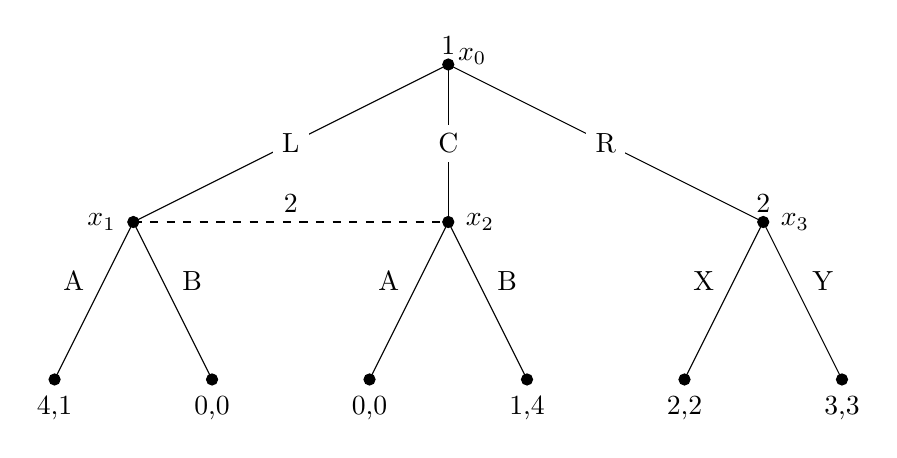
\begin{tikzpicture}
        \filldraw (0,0) circle(2pt)
              (-4,-2) circle (2pt)
              (0,-2) circle (2pt)
              (4,-2) circle (2pt)
              (-5,-4) circle (2pt)
              (-3,-4) circle (2pt)
              (-1,-4) circle (2pt)
              (1,-4) circle (2pt)
              (3,-4) circle (2pt)
              (5,-4) circle (2pt);
        \draw (0,0) -- node[middleweight,fill=white]{L} (-4,-2);
        \draw (0,0) -- node[middleweight,fill=white]{C} (0,-2);
        \draw (0,0) -- node[middleweight,fill=white]{R} (4,-2);
        \draw[dashed] (-4,-2) --node[middleweight,anchor=south]{2}(0,-2);
        \draw (-4,-2) -- node[middleweight,anchor = south east]{A} (-5,-4);
        \draw (-4,-2) -- node[middleweight,anchor = south west]{B}(-3,-4);
        \draw (0,-2) -- node[middleweight,anchor = south east]{A} (-1,-4);
        \draw (0,-2) -- node[middleweight,anchor = south west]{B}(1,-4);
        \draw (4,-2) -- node[middleweight,anchor = south east]{X} (3,-4);
        \draw (4,-2) -- node[middleweight,anchor = south west]{Y}(5,-4);
        \node[anchor = south] at (0,0){1};
        \node[anchor=west] at (0,0.1){$x_0$};
        \node[anchor = east] at (-4.1,-2){$x_1$};
        \node[anchor = west] at (0.1,-2){$x_2$};
        \node[anchor = west] at (4.1,-2){$x_3$};
        \node[anchor = south] at (4,-2){2};
        \node[anchor = north] at (-5,-4.1){4,1};
        \node[anchor = north] at (-3,-4.1){0,0};
        \node[anchor = north] at (-1,-4.1){0,0};
        \node[anchor = north] at (1,-4.1){1,4};
        \node[anchor = north] at (3,-4.1){2,2};
        \node[anchor = north] at (5,-4.1){3,3};
      \end{tikzpicture}
    \end{center}
    \tcblower
    \begin{problem}{(a)}
      Characterize the information sets of the decision nodes (denoted by $x_i$) in this game by writing down all the information sets for each player.
      \tcblower
      \begin{itemize}
        \item Player 1: $\{x_0\}$ (singleton)
        \item Player 2: $\{x_1,x_2\}$ (non-singleton), $\{x_3\}$ (singleton)
      \end{itemize}
    \end{problem}
    \begin{problem}{(b)}
      Write the normal-form game associated with this extensive form game and find all the pure strategy Nash equilibria.
      \tcblower
      % 3x4 normal form game
      \begin{center}
        \begin{tabular}{c|c|c|c|c|}
          \multicolumn{1}{c}{}& \multicolumn{1}{c}{$AX$}& \multicolumn{1}{c}{$AY$}& \multicolumn{1}{c}{$BX$}& \multicolumn{1}{c}{$BY$}\\
          \cline{2-5}
          $L$ & $4,1$ & $4,1$ & $0,0$ & $0,0$\\
          $C$ & $0,0$ & $0,0$ & $1,4$ & $1,4$\\
          $R$ & $2,2$ & $3,3$ & $2,2$ & $3,3$\\
          \cline{2-5}
        \end{tabular}
      \end{center}
      We can see that the Nash equilibria are $(L,AX)$, $(L,AY)$, $(C, BX)$, $(C, BY)$, $(R,AY)$, $(R, BY)$.
    \end{problem}
    \begin{problem}{(c)}
      Which of the Nash equilibria that you found in part (b) are also subgame perfect equilibria?
      \tcblower
      %SPE = Nash Equilibria that are also Nash Equilibria in subgame.
      The Nash equilibria that are also subgame perfect equilibria are the Nash equilibria that are Nash equilibria in the proper subgame starting from $\{x_3\}$. Therefore, the subgame perfect equilibria are:
      \begin{itemize}
        \item $(L, AY)$
        \item $(C, BY)$
        \item $(R, AY)$
        \item $(R, BY)$
      \end{itemize}
    \end{problem}
  \end{problem}
  \begin{problem}{The Shipping News}
    Consider the following extensive form games. In both games, UPS ($U$) has to decide whether to Enter ($E$) or stay out ($O$) of a foreign market where DHL ($D$) is already active. If UPS enters the market, then both firms have to decide whether or not to start a price war by fighting $(F,F^*,f)$ or acquiescing $(A,A^*,a)$ to the entry. The payoffs list that of UPS first, followed by the payoff to DHL.
    \begin{center}
      \begin{tikzpicture}
        \filldraw (0,0) circle (2pt)
                  (-2,-2) circle (2pt)
                  (2,-2) circle (2pt)
                  (0,-4) circle (2pt)
                  (4,-4) circle (2pt)
                  (-1,-6) circle (2pt)
                  (1,-6) circle (2pt)
                  (3,-6) circle (2pt)
                  (5,-6) circle (2pt);
        \draw (0,0) --node[middleweight,anchor=south east]{$O$} (-2,-2);
        \draw (0,0) --node[middleweight,anchor = south west]{$E$} (2,-2);
        \draw (2,-2) --node[middleweight,anchor = south east]{$a$} (0,-4);
        \draw (2,-2) --node[middleweight,anchor = south west] {$f$} (4,-4);
        \draw (0,-4) --node[middleweight, anchor=south east]{$A$} (-1,-6);
        \draw (0,-4) --node[middleweight,anchor = south west]{$F$} (1,-6);
        \draw (4,-4) --node[middleweight, anchor = south east]{$A^*$} (3,-6);
        \draw (4,-4) --node[middleweight,anchor = south west]{$F^*$} (5,-6);
        \node[anchor = south] at (0,0.1) {$U$};
        \node[anchor = south] at (2,-1.9) {$D$};
        \node[anchor = west] at (4.1,-4) {$U$};
        \node[anchor = east] at (-0.1,-4) {$U$};
        \node[anchor = north] at (-2,-2) {0,5};
        \node[anchor = north] at (-1,-6) {1,2};
        \node[anchor = north] at (1,-6) {0,-3};
        \node[anchor = north] at (3,-6) {-3,1};
        \node[anchor = north] at (5,-6) {-2,-1};
      \end{tikzpicture}\\
      \begin{tikzpicture}
        \filldraw (0,0) circle (2pt)
                  (-2,-2) circle (2pt)
                  (2,-2) circle (2pt)
                  (0,-4) circle (2pt)
                  (4,-4) circle (2pt)
                  (-1,-6) circle (2pt)
                  (1,-6) circle (2pt)
                  (3,-6) circle (2pt)
                  (5,-6) circle (2pt);
        \draw (0,0) --node[middleweight,anchor=south east]{$O$} (-2,-2);
        \draw (0,0) --node[middleweight,anchor = south west]{$E$} (2,-2);
        \draw (2,-2) --node[middleweight,anchor = south east]{$a$} (0,-4);
        \draw (2,-2) --node[middleweight,anchor = south west] {$f$} (4,-4);
        \draw (0,-4) --node[middleweight, anchor=south east]{$A$} (-1,-6);
        \draw (0,-4) --node[middleweight,anchor = south west]{$F$} (1,-6);
        \draw (4,-4) --node[middleweight, anchor = south east]{$A$} (3,-6);
        \draw (4,-4) --node[middleweight,anchor = south west]{$F$} (5,-6);
        \draw[dashed] (0,-4) -- node[middleweight,anchor = south]{$U$}(4,-4);
        \node[anchor = south] at (0,0.1) {$U$};
        \node[anchor = south] at (2,-1.9) {$D$};
        \node[anchor = north] at (-2,-2) {0,5};
        \node[anchor = north] at (-1,-6) {1,2};
        \node[anchor = north] at (1,-6) {0,-3};
        \node[anchor = north] at (3,-6) {-3,1};
        \node[anchor = north] at (5,-6) {-2,-1};
      \end{tikzpicture}
    \end{center}
    \tcblower
    \begin{problem}{(a)}
      What is the difference between the two extensive form games with respect to what the players know when they make their decisions?
      \tcblower
      In the first game, UPS only makes its decision to acquiesce or fight after DHL does, but in the second game, UPS and DHL make their decision simultaneously.
    \end{problem}
    \begin{problem}{(b)}
      Write the normal form of both games and find all of the pure strategy Nash equilibria in each game.
      \tcblower
      Sequential Decision:
      \begin{center}
        \small
        \begin{tabular}{cc|c|c|c|c|c|c|c|c|}
          \multicolumn{2}{c}{} & \multicolumn{8}{c}{$U$}\\
          \multicolumn{2}{c}{} & \multicolumn{1}{c}{$OA$}& \multicolumn{1}{c}{$OF$}& \multicolumn{1}{c}{$OA^*$}& \multicolumn{1}{c}{$OF^*$}& \multicolumn{1}{c}{$EA$}& \multicolumn{1}{c}{$EF$}& \multicolumn{1}{c}{$EA^*$}& \multicolumn{1}{c}{$EF^*$}\\
          \cline{3-10}
          \multirow{2}{*}{$D$} & $a$ & $5,0$& $5,0$& $5,0$& $5,0$ & $2,1$ & $-3,0$ & $2,1$ & $-3,0$\\
          \cline{3-10}
                               & $f$ & $5,0$& $5,0$& $5,0$& $5,0$ & $1,-3$ & $-1,-2$ & $1,-3$ & $-1,-2$\\
                               \cline{3-10}
        \end{tabular}
      \end{center}
      The Nash equilibria of this game are as follows:
      \begin{itemize}
        \item $a,EA$
        \item $a,EA^*$
      \end{itemize}
      Simultaneous Decision:
      \begin{center}
        \small
        \begin{tabular}{cc|c|c|c|c|}
          \multicolumn{2}{c}{} & \multicolumn{4}{c}{$U$}\\
          \multicolumn{2}{c}{} & \multicolumn{1}{c}{$OA$}& \multicolumn{1}{c}{$OF$}& \multicolumn{1}{c}{$EA$}& \multicolumn{1}{c}{$EF$}\\
          \cline{3-6}
          \multirow{2}{*}{$D$} & $a$ & $5,0$& $5,0$ & $2,1$ & $-3,0$\\
          \cline{3-6}
                               & $f$ & $5,0$& $5,0$ & $1,-3$ & $-1,-2$\\
                               \cline{3-6}
        \end{tabular}
      \end{center}
      The Nash equilibria is as follows:
      \begin{itemize}
        \item $a,EA$
      \end{itemize}
    \end{problem}
    \begin{problem}{(c)}
      Find all subgame perfect equilibria of both games.
      \tcblower
      The subgame perfect equilibrium of the sequential game is $a,EA$, and the subgame perfect equilibrium of the simultaneous game is $a,EA$.
    \end{problem}
  \end{problem}
  \begin{problem}{Technology Adoption}
    During the adoption of a new technology a CEO (player 1) can design a new task for a division manager. The new task can be either high level ($H$), or low level ($L$). The manager simultaneously chooses to invest in good training ($G$), or bad training ($B$). The payoffs from this interaction are given by the following matrix.
    \begin{center}
      \begin{tabular}{c|c|c|}
        \multicolumn{1}{c}{} & \multicolumn{1}{c}{$G$} & \multicolumn{1}{c}{$B$}\\
        \cline{2-3}
        $H$ & $5,4$ & $-5,2$\\
        \cline{2-3}
        $L$ & $2,-2$ & $0,0$\\
        \cline{2-3}
      \end{tabular}
    \end{center}
    \begin{problem}{(a)}
      Present the game in extensive form and solve for all the Nash equilibria and subgame perfect equilibria.
      \tcblower
      \begin{center}
        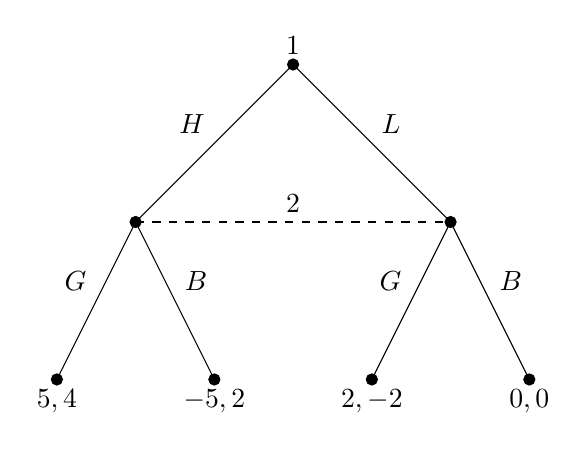
\begin{tikzpicture}
          \filldraw (0,0) circle (2pt)
                    (-2,-2) circle (2pt)
                    (2,-2) circle (2pt)
                    (-3,-4) circle (2pt)
                    (-1,-4) circle (2pt)
                    (1,-4) circle (2pt)
                    (3,-4) circle (2pt);
          \node[anchor = south] at (0,0){$1$};
          \draw (0,0) --node[middleweight,anchor=south east]{$H$} (-2,-2);
          \draw (0,0) --node[middleweight,anchor = south west]{$L$} (2,-2);
          \draw (-2,-2) --node[middleweight,anchor=south east]{$G$} (-3,-4);
          \draw (-2,-2) --node[middleweight,anchor=south west]{$B$} (-1,-4);
          \draw[dashed] (-2,-2) --node[middleweight,anchor=south]{$2$} (2,-2);
          \draw (2,-2) --node[middleweight,anchor=south west]{$B$} (3,-4);
          \draw (2,-2) --node[middleweight,anchor=south east]{$G$} (1,-4);
          \node[anchor = north] at (-3,-4) {$5,4$};
          \node[anchor = north] at (-1,-4) {$-5,2$};
          \node[anchor = north] at (1,-4) {$2,-2$};
          \node[anchor = north] at (3,-4) {$0,0$};
        \end{tikzpicture}
      \end{center}
      There are three Nash equilibria, one at  $(H,G)$, one at $(L,B)$, and one at $\left(\frac{1}{2}H + \frac{1}{2}L,\frac{5}{8}G + \frac{3}{8}B\right)$
    \end{problem}
    \begin{problem}{(b)}
      Assume that before the game is played the CEO can choose not to adopt this new technology, in which case the payoffs are (1,1), or to adopt it, in which the game is played. Present the entire game in extensive form. How many proper subgames does it have?
      \tcblower
      \begin{center}
        \begin{tikzpicture}
          \filldraw (0,0) circle (2pt)
                    (-2,-2) circle (2pt)
                    (2,-2) circle (2pt)
                    (0,-4) circle (2pt)
                    (4,-4) circle (2pt)
                    (-1,-6) circle (2pt)
                    (1,-6) circle (2pt)
                    (3,-6) circle (2pt)
                    (5,-6) circle (2pt);
          \draw (0,0) --node[middleweight,anchor=south east]{$N$} (-2,-2);
          \draw (0,0) --node[middleweight,anchor = south west]{$A$} (2,-2);
          \draw (2,-2) --node[middleweight,anchor = south east]{$H$} (0,-4);
          \draw (2,-2) --node[middleweight,anchor = south west] {$L$} (4,-4);
          \draw (0,-4) --node[middleweight, anchor=south east]{$G$} (-1,-6);
          \draw (0,-4) --node[middleweight,anchor = south west]{$B$} (1,-6);
          \draw (4,-4) --node[middleweight, anchor = south east]{$G$} (3,-6);
          \draw (4,-4) --node[middleweight,anchor = south west]{$B$} (5,-6);
          \draw[dashed] (0,-4) -- node[middleweight,anchor = south]{$2$}(4,-4);
          \node[anchor = south] at (0,0.1) {$1$};
          \node[anchor = south] at (2,-1.9) {$1$};
          \node[anchor = north] at (-2,-2) {1,1};
          \node[anchor = north] at (-1,-6) {5,4};
          \node[anchor = north] at (1,-6) {-5,2};
          \node[anchor = north] at (3,-6) {2,-2};
          \node[anchor = north] at (5,-6) {0,0};
        \end{tikzpicture}
      \end{center}
      There is one proper subgame in this problem, namely the game played earlier.
    \end{problem}
    \begin{problem}{(c)}
      Solve for all the Nash equilibria and subgame perfect equilibria of the game described in (b)
      \tcblower
      The Nash equilibria are $(NL,B)$, $(AH,G)$, and $\left(A,\frac{1}{2}H + \frac{1}{2}L,\frac{5}{8}G + \frac{3}{8}B\right)$, of which $(AH,G)$ and $\left(A,\frac{1}{2}H + \frac{1}{2}L,\frac{5}{8}G + \frac{3}{8}B\right)$ are subgame perfect equilibria.
    \end{problem}
  \end{problem}
  \begin{problem}{Mad Men}
    Two firms (firm 1 and firm 2) producing toothpaste engage in Cournot competition by simultaneously choosing output. The market demand curve is given by
    \begin{align*}
      P = A-Q
    \end{align*}
    where $P$ is price and $Q = q_1 + q_2$ is market output, and $A > 0$ is a constant. Both firms have zero cost of production.
    \begin{problem}{(a)}
      Compute the Nash equilibrium output and profit of each firm in Cournot competition.
      \tcblower
      We know that
      \begin{align*}
        v_i &= q_i \left(A-q_i-q_{-i}\right)\\
        \shortintertext{Therefore, we find $BR_{i}(q_{-i})$ and use symmetry}
         0 &= \frac{\partial v_i}{\partial q_i}\\
         0 &= A - 2q_i - q_{-i}\\
         q_i &= \frac{A-q_{-i}}{2}\\
         q_{i}^* &= \frac{A - q_{i}^*}{2}\tag*{using symmetry}\\
         q_{i}^* &= \frac{A}{3}\\
         v_{i}^* &= \frac{A^2}{9}
      \end{align*}
    \end{problem}
    \begin{problem}{(b)}
      Now interpret $A$ as advertising spent by firm 1. In particular, consider the extensive form modification of the game in which before the two firms engage in Cournot competition, firm 1 chooses a level of advertising, $A$. Firm 2 does not advertise. The cost of advertising at level $A$ is $C(A) = A^3/9$. Find the subgame perfect equilibrium.
      \tcblower
      \begin{align*}
        \shortintertext{Best Response of firm 2:}
        0 &= \frac{\partial v_2}{\partial q_2}\\
        0 &= A - 2q_2 - q_1\\
        BR_{2}(q_1) &= \frac{A-q_1}{2}\\
        \shortintertext{Payoff of firm 1:}
        v_1 &= q_1(A - q_1 - q_2) - A^3/9\\
        0 &= \frac{\partial v_1}{q_1}\\
        0 &= A - 2q_1 - q_2\\
        BR_1(q_2) &= \frac{A - q_2}{2}\\
        \shortintertext{Therefore, we have }
        q_1 &= BR_1(BR_2(q_1))\\
            &= \frac{A}{3}\\
        q_2 &= \frac{A}{3}\\
        \shortintertext{with payoffs of}
        v_1 &= \frac{A^2}{9} - \frac{A^3}{9}\\
        v_2 &= \frac{A^2}{9}
      \end{align*}
      \begin{problem}{Corrections}
        \color{red!50!black}
        Now that we found the payoff for $v_1$, we have to maximize $v_1$ to maximize firm 1's payoff. $A = \frac{2}{3}$, meaning the SPE is:
        \begin{align*}
          A = \frac{2}{3}, q_1(A) = q_2(A) = \frac{A}{3}
        \end{align*}
      \end{problem}
    \end{problem}
  \end{problem}
  \begin{problem}{Resident Assistant Selection with a Twist}
    Two staff managers in the $\Pi $B$ \Phi$ sorority, the house manager (player 1) and kitchen manager (player 2), must select a resident assistant from a pool of three candidates: $\{a,b,c\}$. Player 1 prefers $a$ to $b$ and $b$ to $c$. Player 2 prefers $b$ to $a$ and $a$ to $c$. The process that is imposed on them is as follows:
    \begin{itemize}
      \item First, the house manager vetoes one of the candidates and announces the veto to the central office for staff selection and to the kitchen manager.
      \item Next, the kitchen manager vetoes one of the remaining two candidates and announces it to the central office.
      \item Finally, the director of the central office assigns the remaining candidate to be a resident assistant at $\Pi $B$\Phi$
    \end{itemize}
    \begin{problem}{(a)}
      Model this as an extensive form game, in which a player's most preferred candidate gives a payoff of $2$, the second most preferred candidate gives a payoff of $1$ and the last candidate gives a $0$.
      \tcblower
      In which each label refers to the candidate vetoed, the extensive-form game is as follows:
      \begin{center}
        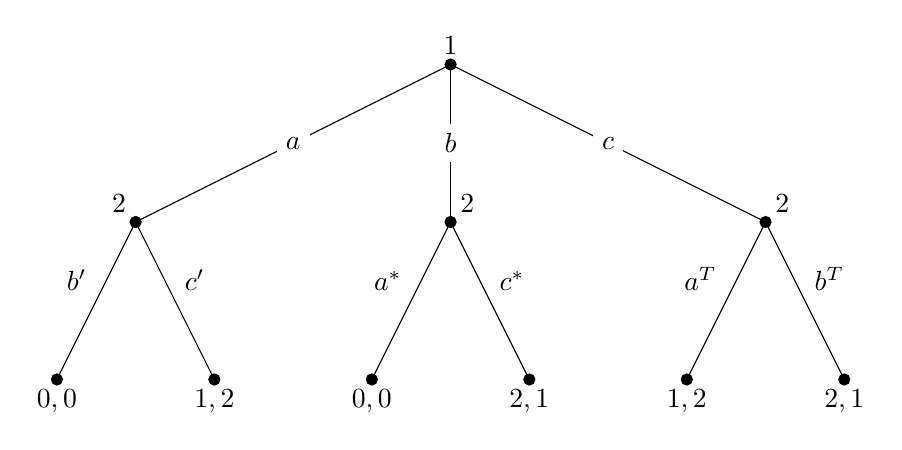
\begin{tikzpicture}
          \filldraw (0,0) circle (2pt)
                    (-4,-2) circle (2pt)
                    (0,-2) circle (2pt)
                    (4,-2) circle (2pt)
                    (-5,-4) circle (2pt)
                    (-3,-4) circle (2pt)
                    (-1,-4) circle (2pt)
                    (1,-4) circle (2pt)
                    (3,-4) circle (2pt)
                    (5,-4) circle (2pt);
          \draw (0,0) -- node[middleweight,fill=white]{$a$} (-4,-2);
          \draw (0,0) --node[middleweight,fill=white]{$b$} (0,-2);
          \draw (0,0)--node[middleweight,fill=white]{$c$}(4,-2);
          \draw (-4,-2)--node[middleweight,anchor = south east]{$b'$} (-5,-4);
          \draw (-4,-2) --node[middleweight,anchor = south west]{$c'$}(-3,-4);
          \draw (0,-2)--node[middleweight,anchor = south east]{$a^*$}(-1,-4);
          \draw (0,-2)--node[middleweight,anchor = south west]{$c^*$}(1,-4);
          \draw (4,-2)--node[middleweight,anchor = south east]{$a^T$}(3,-4);
          \draw (4,-2) --node[middleweight,anchor = south west]{$b^T$}(5,-4);
          \node[anchor = south] at (0,0) {$1$};
          \node[anchor = south west] at (4,-2) {$2$};
          \node[anchor = south east] at (-4,-2){$2$};
          \node[anchor = south west] at (0,-2){$2$};
          \node[anchor = north] at (-5,-4) {$0,0$};
          \node[anchor = north] at (-3,-4) {$1,2$};
          \node[anchor = north] at (-1,-4) {$0,0$};
          \node[anchor = north] at (1,-4) {$2,1$};
          \node[anchor = north] at (3,-4) {$1,2$};
          \node[anchor = north] at (5,-4) {$2,1$};
        \end{tikzpicture}
      \end{center}
    \end{problem}
    \begin{problem}{(b)}
      Find the subgame perfect equilibrium for this game. Is it unique?
      \tcblower
      The subgame perfect equilibrium is $(b,c'c^*a^T)$. This subgame perfect equilibrium is unique as it is a Nash equilibrium in both one of the subgames and in the larger game.
    \end{problem}
    \begin{problem}{(c)}
      Are there Nash equilibria that are not subgame perfect equilibria?
      \tcblower
      Each of the Nash equilibria in each subgame is a Nash equilibrium, meaning there are Nash equilibria that are not subgame perfect equilibria.
    \end{problem}
    \begin{problem}{(d)}
      Now assume that before the two players play the game, player 2 can send an alienating email to one of the candidates, which would result in that candidate withdrawing their application. Would player choose to do this, and if so, with which candidate?
      \tcblower
      Player 2 would choose to send the email to candidate $a$, as that would effectively cause this game to go to the leftmost subgame in the above game tree, in which player 1 would choose to veto $c$'s candidacy, meaning player 2 would receive their first choice candidate, $b$, as the resident assistant.
    \end{problem}
  \end{problem}
\end{document}
